% A LaTeX template for EXECUTIVE SUMMARY of the MSc Thesis submissions to 
% Politecnico di Milano (PoliMi) - School of Industrial and Information Engineering
%
% S. Bonetti, A. Gruttadauria, G. Mescolini, A. Zingaro
% e-mail: template-tesi-ingind@polimi.it
%
% Last Revision: October 2021
%
% Copyright 2021 Politecnico di Milano, Italy. NC-BY

\documentclass[11pt,a4paper,twocolumn]{article}

%------------------------------------------------------------------------------
%	REQUIRED PACKAGES AND  CONFIGURATIONS
%------------------------------------------------------------------------------
% PACKAGES FOR TITLES
\usepackage{titlesec}
\usepackage{color}

% PACKAGES FOR LANGUAGE AND FONT
\usepackage[utf8]{inputenc}
\usepackage[english]{babel}
\usepackage[T1]{fontenc} % Font encoding

% PACKAGES FOR IMAGES
\usepackage{graphicx}
\graphicspath{{Configuration_Files/Images/}} % Path for images' folder
\usepackage{eso-pic} % For the background picture on the title page
\usepackage{subfig} % Numbered and caption subfigures using \subfloat
\usepackage{caption} % Coloured captions
\usepackage{transparent}

% STANDARD MATH PACKAGES
\usepackage{amsmath}
\usepackage{amsthm}
\usepackage{bm}
\usepackage{dsfont}
\usepackage[overload]{empheq}  % For braced-style systems of equations

% PACKAGES FOR TABLES
\usepackage{tabularx}
\usepackage{longtable} % tables that can span several pages
\usepackage{colortbl}

% PACKAGES FOR ALGORITHMS (PSEUDO-CODE)
\usepackage{algorithm}
\usepackage[linesnumbered,ruled,noend,algo2e]{algorithm2e}

% PACKAGES FOR REFERENCES & BIBLIOGRAPHY
\usepackage[colorlinks=true,linkcolor=black,anchorcolor=black,citecolor=black,filecolor=black,menucolor=black,runcolor=black,urlcolor=black]{hyperref} % Adds clickable links at references
\usepackage{cleveref}
\usepackage[square, numbers, sort&compress]{natbib} % Square brackets, citing references with numbers, citations sorted by appearance in the text and compressed
\bibliographystyle{plain} % You may use a different style adapted to your field

% PACKAGES FOR THE APPENDIX
\usepackage{appendix}

% PACKAGES FOR ITEMIZE & ENUMERATES 
\usepackage{enumitem}

% OTHER PACKAGES
\usepackage{amsthm,thmtools,xcolor} % Coloured "Theorem"
\usepackage{comment} % Comment part of code
\usepackage{fancyhdr} % Fancy headers and footers
\usepackage{lipsum} % Insert dummy text
\usepackage{tcolorbox} % Create coloured boxes (e.g. the one for the key-words)
\usepackage{stfloats} % Correct position of the tables

%-------------------------------------------------------------------------
%	NEW COMMANDS DEFINED
%-------------------------------------------------------------------------
% EXAMPLES OF NEW COMMANDS -> here you see how to define new commands
\newcommand{\bea}{\begin{eqnarray}} % Shortcut for equation arrays
\newcommand{\eea}{\end{eqnarray}}
\newcommand{\e}[1]{\times 10^{#1}}  % Powers of 10 notation
\newcommand{\mathbbm}[1]{\text{\usefont{U}{bbm}{m}{n}#1}} % From mathbbm.sty
\newcommand{\pdev}[2]{\frac{\partial#1}{\partial#2}}
% NB: you can also override some existing commands with the keyword \renewcommand
\theoremstyle{definition}
\newtheorem{definition}{Definition}[section]
\newcommand{\kpub}{\ensuremath{\mathcal{K}_{pub}}}
\newcommand{\kpri}{\ensuremath{\mathcal{K}_{pri}}}
\newcommand{\sample}{\ensuremath{ \stackrel{\$}{\gets} }}
\newcommand{\ssplit}[1]{\ensuremath{ \llbracket #1 \rrbracket }}
\newcommand{\clshift}{\ensuremath{\lll_n}}


\usepackage{amssymb}
\usepackage{booktabs}
\usepackage{tikz}
\usepackage{pgfplots}
\usepackage{pgfplotstable}
\pgfplotsset{compat=1.16}
\usetikzlibrary{positioning}
\usetikzlibrary{patterns}
\usepackage{stmaryrd}
\usepackage{multicol} % To write in multiple columns (executive summary)
\usepackage{multirow}

%----------------------------------------------------------------------------
%	ADD YOUR PACKAGES (be careful of package interaction)
%----------------------------------------------------------------------------


%----------------------------------------------------------------------------
%	ADD YOUR DEFINITIONS AND COMMANDS (be careful of existing commands)
%----------------------------------------------------------------------------


% Do not change Configuration_files/config.tex file unless you really know what you are doing. 
% This file ends the configuration procedures (e.g. customizing commands, definition of new commands)
% Set the geometric layout of the document
\usepackage{geometry}
\geometry{
  top=3cm,
  left = 2.0cm,
  right = 2.0cm,
  bottom=2cm,
  headheight= 2cm,
  headsep= 0cm,
}
\raggedbottom 

% Create color bluePoli (-> manuale grafica coordinata:  https://www.polimi.it/fileadmin/user_upload/il_Politecnico/grafica-coordinata/2015_05_11_46xy_manuale_grafica_coordinata.pdf)
\definecolor{bluePoli}{cmyk}{0.4,0.1,0,0.4}

% Custom theorem environments
\declaretheoremstyle[
  headfont=\color{bluePoli}\normalfont\bfseries,
  bodyfont=\color{black}\normalfont\itshape,
]{colored}

\captionsetup[figure]{labelfont={color=bluePoli}} % Set colour of the captions
\captionsetup[table]{labelfont={color=bluePoli}} % Set colour of the captions
\captionsetup[algorithm]{labelfont={color=bluePoli}} % Set colour of the captions

\theoremstyle{colored}
\newtheorem{theorem}{Theorem}[section]
\newtheorem{proposition}{Proposition}[section]

% Enhances the features of the standard "table" and "tabular" environments.
\newcommand\T{\rule{0pt}{2.6ex}}
\newcommand\B{\rule[-1.2ex]{0pt}{0pt}}

% Algorithm description
\newcounter{algsubstate}
\renewcommand{\thealgsubstate}{\alph{algsubstate}}
\newenvironment{algsubstates}{
    \setcounter{algsubstate}{0}%
    \renewcommand{\STATE}{%
    \stepcounter{algsubstate}%
    \Statex {\small\thealgsubstate:}\space}
    }{}
    
% Custom theorem environment
\newcolumntype{L}[1]{>{\raggedright\let\newline\\\arraybackslash\hspace{0pt}}m{#1}}
\newcolumntype{C}[1]{>{\centering\let\newline\\\arraybackslash\hspace{0pt}}m{#1}}
\newcolumntype{R}[1]{>{\raggedleft\let\newline\\\arraybackslash\hspace{0pt}}m{#1}}

% Custom itemize environment
\setlist[itemize,1]{label=$\bullet$}
\setlist[itemize,2]{label=$\circ$}
\setlist[itemize,3]{label=$-$}
\setlist{nosep}

% Set separation of columns 
\setlength{\columnsep}{30pt}

% Create command for background pic
\newcommand\BackgroundPic{% Adding background picture
	\put(230,358){
		\parbox[b][\paperheight]{\paperwidth}{%
			\vfill
			\centering
			\transparent{0.4}
			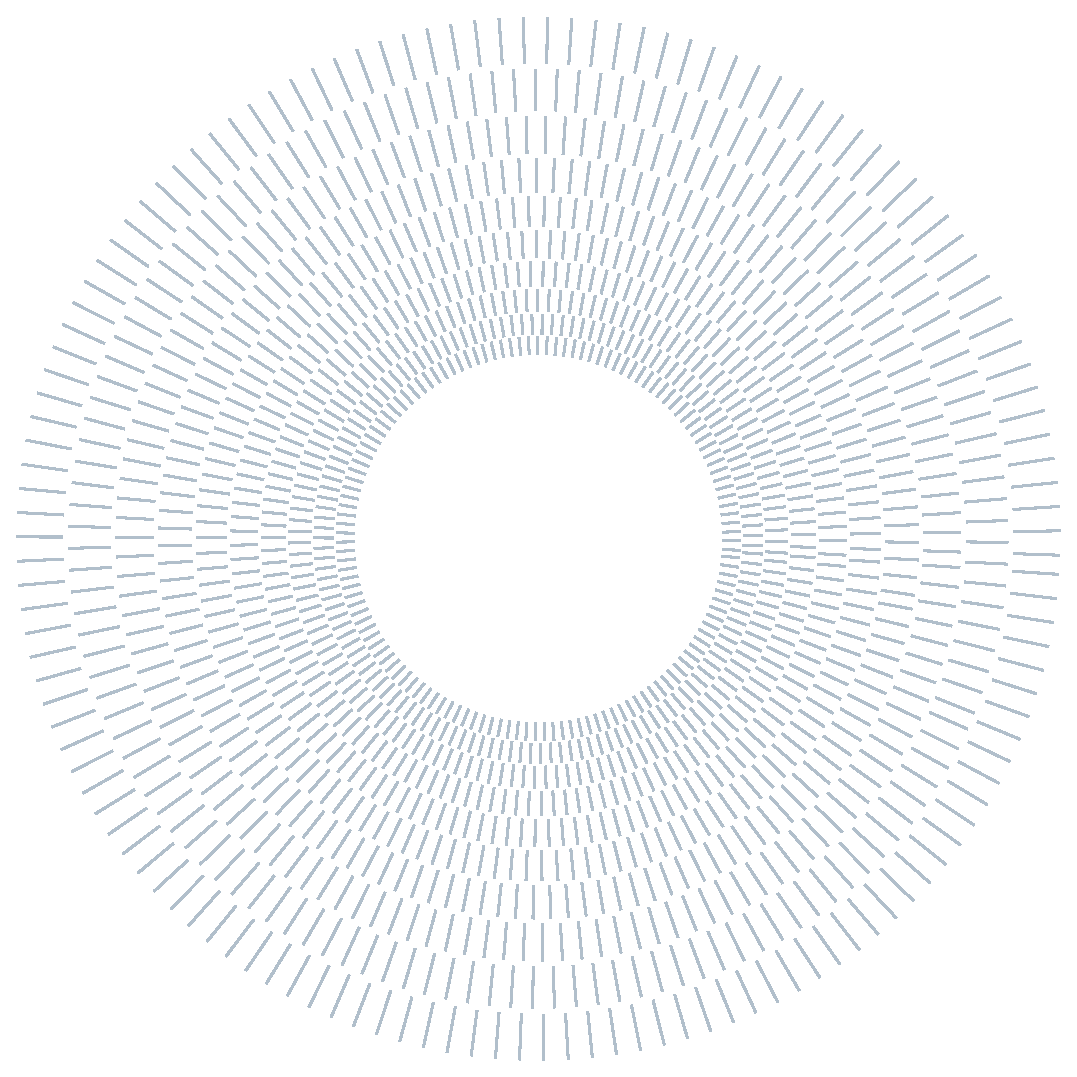
\includegraphics[width=0.5\paperwidth]{raggiera_polimi.eps}%
			\vfill
}}}

% Set indentation
\setlength\parindent{0pt}

% Custom title commands
\titleformat{\section}
{\color{bluePoli}\normalfont\Large\bfseries}
{\color{bluePoli}\thesection.}{1em}{}
\titlespacing*{\section}
{0pt}{2ex}{1ex}

\titleformat{\subsection}
{\color{bluePoli}\normalfont\large\bfseries}
{\color{bluePoli}\thesubsection.}{1em}{}
\titlespacing*{\subsection}
{0pt}{2ex}{1ex}

% Custom headers and footers
\pagestyle{fancy}
\fancyhf{}
      
\fancyfoot{}
\fancyfoot[C]{\thepage} % page
\renewcommand{\headrulewidth}{0mm} % headrule width
\renewcommand{\footrulewidth}{0mm} % footrule width

\makeatletter
\patchcmd{\headrule}{\hrule}{\color{black}\hrule}{}{} % headrule
\patchcmd{\footrule}{\hrule}{\color{black}\hrule}{}{} % footrule
\makeatother

% -> Create the header
\chead[C]{
\centering
\begin{tcolorbox}[arc=0pt, boxrule=0pt, colback=bluePoli!60, width=\textwidth, colupper=white]
    \textbf{Executive summary} \hfill \textbf{\author}  
\end{tcolorbox}
}

% Insert here the info that will be displayed into your Title page 
% -> title of your work
\renewcommand{\title}{Towards fast and side-channel resistant implementations of \\Hamming Quasi-Cyclic: a case study on ARM Cortex-M4 devices}
% -> author name and surname
\renewcommand{\author}{Domenico Cacace}
% -> MSc course
\newcommand{\course}{Computer Engineering - Ingegneria Informatica}
% -> advisor name and surname
\newcommand{\advisor}{Prof. Alessandro Barenghi}
% IF AND ONLY IF you need to modify the co-supervisors you also have to modify the file Configuration_files/title_page.tex (ONLY where it is marked)
\newcommand{\firstcoadvisor}{Prof. Gerardo Pelosi} % insert if any otherwise comment
%\newcommand{\secondcoadvisor}{Name Surname} % insert if any otherwise comment
% -> academic year
\newcommand{\YEAR}{2022-2023}

%-------------------------------------------------------------------------
%	BEGIN OF YOUR DOCUMENT
%-------------------------------------------------------------------------
\begin{document}

%-----------------------------------------------------------------------------
% TITLE PAGE
%-----------------------------------------------------------------------------
% Do not change Configuration_files/TitlePage.tex (Modify it IF AND ONLY IF you need to add or delete the Co-advisors)
% This file creates the Title Page of the document
% DO NOT REMOVE SPACES BETWEEN LINES!

\twocolumn[{\begin{@twocolumnfalse}

    \AddToShipoutPicture*{\BackgroundPic}
    
    \hspace{-0.6cm}
\includegraphics[width=0.6\textwidth]{logo_polimi_ing_indinf.eps}
    
    \vspace{-1mm}
    \fontsize{0.3cm}{0.5cm}\selectfont \bfseries \textsc{\color{bluePoli} Executive Summary of the Thesis}\\
    
    \vspace{-0.2cm}
    \Large{\textbf{\color{bluePoli}{\title}}}\\
    
    \vspace{-0.2cm}
    \fontsize{0.3cm}{0.5cm}\selectfont \bfseries \textsc{\color{bluePoli} Laurea Magistrale in \course}\\
    
    \vspace{-0.2cm}
    \fontsize{0.3cm}{0.5cm} \selectfont \bfseries Author: \textsc{\textbf{\author}}\\
    
    \vspace{-0.4cm}
    \fontsize{0.3cm}{0.5cm}\selectfont \bfseries Advisor: \textsc{\textbf{\advisor}}\\
    
    % if only ONE co-advisor is present:
    \vspace{-0.4cm}
    \fontsize{0.3cm}{0.5cm}\selectfont \bfseries Co-advisor: \textsc{\textbf{\firstcoadvisor}}\\
    % if more than one co-advisors are present:
    %\vspace{-0.4cm}
    %\fontsize{0.3cm}{0.5cm}\selectfont \bfseries Co-advisors: \textsc{\textbf{\firstcoadvisor}}\textsc{\textbf{\secondcoadvisor}}\\
    
    \vspace{-0.4cm}
    \fontsize{0.3cm}{0.5cm}\selectfont \bfseries Academic year: \textsc{\textbf{\YEAR}}
    
    \small \normalfont
    
    \vspace{11pt}
    
    \centerline{\rule{1.0\textwidth}{0.4pt}}
    
    \vspace{15pt}
    \end{@twocolumnfalse}}]
    
    \thispagestyle{plain} % In order to not show the header in the first page

%%%%%%%%%%%%%%%%%%%%%%%%%%%%%%
%%     THESIS MAIN TEXT     %%
%%%%%%%%%%%%%%%%%%%%%%%%%%%%%%

%-----------------------------------------------------------------------------
% INTRODUCTION
%-----------------------------------------------------------------------------
\section{Introduction}
\label{sec:introduction}
The advancements in quantum computing threaten the \emph{status quo} in 
the cryptography field: a quantum computer with a sufficient amount of
qubits is able, thanks to Shor's algorithm,
to break most of the current public key cryptosystems in polynomial time.\\
For this reason in 2016 the National Institute of Standards and Technologies (NIST)
launched a competition with the aim of developing and standardizing one or more
quantum-resistant cryptosystems. After three rounds CRYSTALS-Kyber, a lattice-based
cryptosystem, was selected as standardization candidate; however, in the event of a potentially
disruptive attack on lattice-based cryptosystems, NIST decided to further extend the competition
selecting four more candidates that rely on different hard problems. Excluding SIKE, the remaining
candidates, namely BIKE, HQC and Classic McEliece
are all based on the hardness of the syndrome decoding problem.\\
The object of this work is HQC~\cite{melchor2018hamming}, a code-based cryptosystem whose
security relies on the syndrome decoding problem for quasi-cyclic codes. HQC comprises both a Public Key
Encryption (PKE) scheme and a Key Encapsulation Mechanism (KEM), obtained by applying the HHK Fujisaki-Okamoto 
transformation on the former.

\paragraph{Related work} Given the sound security record of HQC, much attention has been devoted to its side-channel
resistance. Most of the independent analyses focus on extracting information from electromagnetic and power traces,
whilst at the end of Round 2 of the NIST contest two timing attack that takes advantage of the non constant-time implementation of the BCH decoder have been shown; these attacks are no longer relevant,
as the authors of HQC swapped the BCH code with a Reed-Muller Reed-Solomon concatenated code, implementing a constant-time decoder.
Nontheless a new timing attack has been discovered, which exploits a weakness in the
\emph{rejection sampling} procedure, employed to generate random sparse polynomials; as a countermeasure, a more care careful implementation
of the rejection sampling procedure has been implemented in Round 4, fixing the issue.\\
To date, no dedicated constant-time implementation of HQC targeting embedded systems has been proposed, despite the fact that side channel attacks
are easier to carry on such platforms. The current state of software implementations of HQC tailored for the ARM Cortex-M4 microcontroller, chosen
by the NIST as the reference platform for microcontroller benchmarks, includes only the one in PQM4, a third-party
public project that collects the implementations of NIST Round 4 candidates tailored for Cortex-M4. The latest version of HQC in PQM4 is directly
derived from the Round 3 reference implementation, with no optimizations: as a consequence, this implementation is not constant-time and 
vulnerable to the timing attack presented in~\cite{DBLP:journals/tches/GuoHJLNS22}.

\paragraph{Our contribution} In this work we present the first fully constant-time
software implementation of HQC, together with a comparative analysis of constant-time
binary polynomial multiplication techniques, both tailored for ARM Cortex-M4 microprocessors.
We provide an experimental validation of the constant-time properties via a battery of statistical
t-tests, while varying the CPU frequency to highlight the stability of our solution across
different memory access latencies. Our results show that the optimal solution for the target 
platform is a FFT-based approach, in contrast with classic divide-et-impera techniques
(\emph{i.e.} Karatsuba) which provide better performance on x86 architectures.\\
Moreover, to counter power attacks, we propose a masking scheme that can be applied to the
entire cryptosystem, presenting our results on its potential efficacy.
Finally, we compare our work with the latest implementations available of
BIKE and Classic McEliece, showing the high efficiency of our approaches.

\section{Background}
\label{sec:background}
In this section we lay the theoretical foundations required to understand our work.
To avoid confusion, throughout this work we will use the following notation, unless specified otherwise.
Capital bold letters ($\mathbf{A}, \mathbf{B}, \cdots$) denote generic sets, while lowercase
bold letters ($\mathbf{v}, \mathbf{w}, \cdots$) denote vectors. Binary Galois fields of dimension $n$ are denoted
by $\mathds{F}_{2^n}$ or $GF(2^n)$, while the vector space of dimension $n$ over the field $GF(2)$ is denoted by
either $\mathds{F}_2^n$ or $\mathcal{V}$. The ring of binary polynomials modulo $(x^n-1)$ is denoted by $\mathcal{R}$; 
the value of $n$ is chosen in such a way that the algebra in the ring $\mathcal{R}$ is isomorphic to the algebra
of binary $n\times n$ circulant matrices.

\subsection{Polynomial multiplication}
The most expensive operation in terms of execution time in our cryptosystem is, by far, the polynomial multiplication:
it is thus essential to choose a fast algorithm in order to increase the overall performance.

\subsubsection{Karatsuba Multiplication}
One of the most known fast multiplication algorithms is Karatsuba. This is a divide-et-impera algorithm, which
splits the $n$-degree input polynomials into smaller $m$-degree ones:
\begin{equation*}
    a(x) = a_0(x) +x^m\cdot a_1(x)
\end{equation*}
With the operands in this form, it is possible to rewrite the product of two polynomials as
\begin{equation*}
    c(x) = z_2(x)\cdot x^{2m}+z_1(x)\cdot x^m + z_0(x)
\end{equation*}
with
\begin{equation*}
    \begin{aligned}
        z_2(x) &= a_1(x)b_1(x)\\
        z_1(x) &= a_1(x)b_0(x) + a_0(x)b_1(x)\\
        z_0(x) &= a_0(x)b_0(x)
    \end{aligned}
\end{equation*}
Karatsuba observed that, at the cost of a few more additions, it is possible to calculate
the product using only three multiplications by rewriting $z_1$ as
\begin{equation*}
    (a_0(x)+a_1(x))(b_0(x)+b_1(x))-z_0(x)-z_2(x)
\end{equation*}
This trick allows to calculate the product, under the assumption that $m = \lceil n/2 \rceil$, 
with $\mathcal{O}(n^{\log_2 3})$ operations.

\subsubsection{Frobenius Additive FFT}
Instead of multiplying two polynomials (of degree less than $n$) directly, we can:
\begin{itemize}
    \item Sample the polynomials at $2n+1$ distinct points ($a(i), b(i)$)
    \item Perform the pointwise multiplication of the samples ($c(i) = a(i)b(i)$)
    \item Interpolate the points to get the product of the original polynomials
\end{itemize}
This approach may appear slower than the schoolbook method, as the sampling requires $\mathcal{O}(n^2)$ operations,
the pointwise product $\mathcal{O}(n)$ and the interpolation up to $\mathcal{O}(n^3)$ with the Gauss elimination method. 
However, by recursively splitting the operands and by picking a set of \emph{special} point, such as the $n$-th roots of unity in $\mathds{C}$, 
the sampling and interpolation steps can be performed with the Discrete Fourier Transform and its inverse:
algorithms that perform this procedure are commonly called Fast Fourier Transforms (FFTs), and can achieve a
complexity of $\mathcal{O}(n \log{n})$ operations.

Fields of characteristic two usually do not admit non-trivial roots of unity; nontheless, we can apply the same
principle by picking as evaluation points the powers of a primitive element of the field: these algorithms are called
Additive FFTs.
An example of Additive FFT is the Lin-Chung-Han (LCH) FFT which, for polynomials of degree
$n=2^m$, calculates the product in $\mathcal{O}(n\log{n})$.

\paragraph{New polynomial basis} In~\cite{DBLP:journals/tit/GaoM10} Gao and Mateer use a special basis to
represent the polynomials for their FFT. For polynomials of degree $n=2^m$, the Cantor basis $\mathbf{v} = (v_1, \cdots, v_m)$
of $\mathds{F}_2^m$ follows the structure:
\begin{equation*}
    v_1 = 1, \qquad v_i^2+v_i = v_{i-1} \text{  for } i > 1
\end{equation*}
With respect to this basis we can define a sequence of \emph{nested} subspaces:
\begin{equation*}
    \mathbf{W}_i := span\{v_0, \cdots, v_{i-1}\}, \quad \mathbf{W}_0 \subset \cdots \subset \mathds{F}_2^m
\end{equation*}
and, for each subspace, its vanishing polynomial:
\begin{equation*}
    s_i(x) = \prod_{a \in \mathbf{W}_i}(x-a)
\end{equation*}
For the LCH FFT we first need to represent the polynomials in a different basis, built onto the vanishing polynomials;
this basis ($X_1, \cdots, X_{n-1}$) is called \emph{novelpoly basis}, and is defined as:
\begin{equation*}
    X_k(x) = \prod(s_i(x))^{b_i} \quad \text{ with } k=\sum_{i=0}^{\log_2 n}b_i2^i
\end{equation*}

\paragraph{The butterflies}
As with other FFT, in the LCH FFT we recursively split the input polynomial into two halves; we also split the 
set of evaulation points $\mathbf{W}_k$ into two disjoint sets, $\mathbf{W}_{k-1}$ and $\mathbf{W}_k \setminus \mathbf{W_{k-1}} = \{x+v_k|x\in \mathbf{W}_{k-1}\}$.
Because of the linearity of the vanishing polynomial ($s_i(x+y) = s_i(x)+s_i(y)$), the evaluations of the input polynomial at
$\mathbf{W}_k \setminus \mathbf{W_{k-1}}$ can be quickly computed from the evaluations at $\mathbf{W}_{k-1}$ with the \textit{butterfly} operation,
shown at lines \ref{line:h0} and \ref{line:h1} in Algorithm~\ref{alg:fft}

\begin{algorithm2e}
    \caption{Lin-Chung-Han FFT}
    \label{alg:fft}
    \KwIn{$f(x)$, in novelpoly basis,\newline
            $\alpha \in \mathds{F}_{2^m}$, a generic field element}
    \KwOut{$\{f(x) | x \in \mathbf{W}_m\}$}
    \SetKwFunction{fft}{\textsc{FFT}}
    \SetKwProg{Fn}{Function}{}{}

    \Fn{\fft{$f(x), \alpha$}}{
        \If{$\deg(f(x))$}{
            \KwRet{$[g_0]$}\;
        }
        $k \gets \max{i} \text{ s.t. } 2^i \leq \deg(f(x))$\;
        $g(X) \gets p_0(X) + X_{2^k}\cdot p_1(X)$\;
        $h_0(X) \gets p_0(X) + s_k(\alpha)\cdot p_1(X)$\;\label{line:h0}
        $h_1(X) \gets h_0(X) + s_k(v_k)\cdot p_1(X)$\;\label{line:h1}
        \KwRet{\fft{$h_0(X), \alpha$}, \fft{$h_1(X), v_{k}+\alpha$}}\;
    }
\end{algorithm2e}
Notice that the butterfly carries out two field additions but only one field multiplication,
because $s_k(v_k)=1$ in Cantor basis (\cite{DBLP:journals/corr/abs-1708-09746}, Appendix A).
The output of this algorithm is the set of evaluation points of the input polynomial; these can be multiplied
with the evaluations of a second polynomial and, by performing the FFT and basis conversion backwards, we can
obtain the product of the two.

\paragraph{Frobenius partition}
In~\cite{DBLP:conf/issac/HoevenL17} the authors showed that, by applying the Frobenius map ($\phi: x \mapsto x^2$),
it is possible to derive more values of a polynomial from less evaluation points: 
given a polynomial $f(x)$ of degree at most $n$, we can design a set of points
$\mathbf{S} \subset \mathds{F}_{2^m}$ for $m$ power of 2 such that we can derive $n$ evaluations
of $f$ from $\mathbf{S}$. In~\cite{DBLP:conf/issac/LiCKCY18} the authors suggest to pick $\mathbf{S}$ as:
\begin{equation}
    \mathbf{S} := v_{l+m/2}+\mathbf{W}_l = \{v_{l+m/2}+x | x \in \mathbf{W}_l\}
    \label{eq:frobpart}
\end{equation}
with $l = \log_2 n - \log_2 m$ and size $n^\prime = |\mathbf{S}| = |\mathbf{W}_l| = 2^l = n/m$.
As explained by the authors, this construction allows to reach $n$ points in $\mathds{F}_{2^m}$ by applying
the Frobenius map, which also ensures that the evaluation function
\begin{equation*} 
    E_\mathbf{S}: f(x) \mapsto f(\mathbf{S}) = \{f(v_{l+m/2+w}) | w \in \mathbf{W}_l\}
\end{equation*}
will be invertible.

\subsection{Side-channel attacks}
Even though a cryptographic primitive may be secure from a theoretical point of view, 
its implementation may not. It is possible that a device exposes some \emph{side channels}, 
observable aspects of a system that may reveal information about the internal state of the system;
these side channels, if the device runs a cryptosystem, be exploited to \emph{leak} secret information, such
as a message or the keys employed to decrypt it.

Two of the most common side-channel attacks, especially on embedded devices, are:
\begin{itemize}
    \item \textbf{Timing attacks}: the execution time of an operation may depend on the values of its inputs, allowing
    an attacker to retrieve information by measuring the execution time
    \item \textbf{Power attacks}: the amount of power required by the CPU varies based on the workload, which directly
    depends on the operations being run and their inputs
\end{itemize}

The presence of a side channel does not necessarily mean that an attack is possible,
as the leaked information may not be sufficient to succesfully exfiltrate information.
If this is not the case, there are various countermeasures to mitigate the risk of a successful attack,
such as:

\begin{itemize}
    \item Constant-time algorithms: running an operation takes always the same amount of time, regardless of the
    input (\emph{e.g.} substitute branching instructions depending on the inputs)
    \item Masking: randomize the inputs of an algorithm without affecting the outputs; this can be achieved by
    splitting sensitive data $x$ into $d+1$ \emph{shares}, such that $x = x_0 \oplus \cdots \oplus x_d$,
    making the sensitive value indistinguishable from random noise.
\end{itemize}



\subsection{Coding theory}
To better understand how HQC works, we now give the basic concepts of coding theory.
\begin{definition}[Circulant matrix]
    Let $\mathbf{v} = (v_0, \cdots, v_{n-1}) \in \mathcal{V}$. The circulant matrix induced by $\mathbf{v}$ is defined as
    a matrix whose $i$-th row is the vector $\mathbf{v}$ shifted by $i$ positions to the right:
    \begin{equation*}
        \mathbf{circ(v)} = \begin{pmatrix}
            v_0 & v_1 & \cdots & v_{n-1} \\
            v_{n-1} & v_0 & \cdots & v_{n-2} \\
            \vdots & \vdots & \ddots & \vdots \\
            v_1 & v_2 & \cdots & v_0
            \end{pmatrix} \in \mathds{F}_2^{n\times n}
    \end{equation*}
\end{definition}
The algebra of $n\times n$ circulant matrices over $\mathds{F}_2$ is isomorphic to the algebra of polynomials
in the ring $\mathcal{R}$


\begin{definition}[Linear Codes]
    A linear code $\mathcal{C}$ of lenght $n$ and dimension $k$ (denoted as $[n, k]$) is a subspace of $\mathcal{V}$ 
    of dimension $k$; the elements of $\mathcal{C}$ are called \textit{codewords}.\\
    Due to the linearity of $\mathcal{V}$, any linear combination of two codewords is also a codeword.
\end{definition}

\begin{definition}[Generator Matrix]
    Let $\mathcal{C} = [n,k]$ be a linear code. The matrix $\mathbf{G} \in \mathds{F}_2^{k\times n}$ is called the generator 
    matrix of $\mathcal{C}$ if
    \begin{equation*}
        \mathcal{C} = \{\mathbf{mG}, \text{ for } \mathbf{m}\in \mathds{F}_2^k\}
    \end{equation*}
\end{definition}

\begin{definition}[Parity-Check Matrix]
    Let $\mathcal{C} = [n,k]$ be a linear code. The matrix $\mathbf{H} \in \mathds{F}_2^{(n-k)\times n}$ is called the 
    parity-check matrix of $\mathcal{C}$ if
    \begin{equation*}
        \mathcal{C} = \{\mathbf{v} \in \mathds{F}_2^n \text{ such that } \mathbf{Hv}^\top = 0\}
    \end{equation*}
    In other words, $\mathbf{H}$ is the generator matrix of the dual code $\mathcal{C}^\perp$.
\end{definition}

\begin{definition}[Syndrome]
    Let $\mathcal{C} = [n,k]$ be a code, $\mathbf{H}$ its parity matrix and $\mathbf{v} \in \mathds{F}_2^n$ a word. 
    The syndrome of $\mathbf{v}$ is defined as
    \begin{equation*}
        \mathbf{S}(\mathbf{v}) = \mathbf{Hv}^\top
    \end{equation*}
    From this definition,  a vector $\mathbf{v}$ is a codeword if and only if its syndrome is the zero vector.
\end{definition}

\begin{definition}[Quasi-Cyclic Codes]
    Let $\mathbf{c} = (\mathbf{c}_0, \cdots, \mathbf{c}_{s-1}) \in \mathds{F}_2^{sn}$ be a vector, where we consider 
    each $\mathbf{c}_i$ as a vector in $\mathds{F}_2^n$.
    A linear code $\mathcal{C} = [sn,k]$ is Quasi-Cyclic of index $s$ if, for any $\mathbf{c} \in \mathcal{C}$, 
    the vector obtained by applying a circular shift to every block $\mathbf{c}_i$ simultaneously is also a codeword.
\end{definition}

\subsubsection{Hard problems for cryptography}
The problems we are interested in are all variants of the \textit{decoding problem}, which requires to find 
the closest codeword to a given word with respect to a certain metric; in our case we consider as metric the Hamming
weight, denoted as \texttt{wt}($\mathbf{v}$), which is the amount of non-zero coordinates of the vector $\mathbf{v}$.
In the case of linear codes we have shown that the decoding problem stays the same whether one is given 
the syndrome of the received vector or the vector itself; for this reason, we will only consider 
the \textit{Syndrome Decoding} (\textsf{SD}) problem.\\

\begin{definition}[\textsf{SD} Distribution]
    Given $n,k,w \in \mathds{N}$, the distribution $\textsf{SD}(n, k, w)$ randomly samples a parity-check matrix 
    $\mathbf{H} \xleftarrow{\mathdollar} \mathds{F}_2^{(n-k)\times n}$, a vector 
    $\mathbf{x} \xleftarrow{\mathdollar} \mathds{F}_2^n$ such that $\texttt{wt}(\mathbf{x}) = w$ 
    and returns ($\mathbf{H}, \mathbf{S}(\mathbf{x})$).
\end{definition}

\begin{definition}[\textsf{SD} Problem]
    Given $(\mathbf{H}, \mathbf{y}^\top) \in \mathds{F}_2^{(n-k)\times n} \times \mathds{F}_2^{(n-k)}$ from the $\textsf{SD}(n, k, w)$ 
    distribution, the \textsf{SD} problem requires to find a vector $\mathbf{x} \in \mathds{F}_2^n$ such that 
    $\mathbf{S}(\mathbf{x}) = \mathbf{y}^\top$ and $\texttt{wt}(\mathbf{x}) = w$.
\end{definition}
This problem has been proven to be NP-complete.

\subsection{Hamming Quasi-Cyclic}
    Hamming Quasi-Cyclic is a code-based cryptosystem, that includes both a public-key
    encryption scheme and a key encapsulation mechanism. The KEM is built by applying the HHK
    transformation on the PKE, hence we will focus on the latter.
    HQC employs two different codes:
    \begin{itemize}
        \item A public decodable code $\mathcal{C}$ generated by $\mathbf{G}$ which can correct
        up to $\delta$ errors efficiently with $\mathcal{C}$.\textsf{Decode}().
        \item A random code with parity-check matrix $\mathbf{H} = [\mathbf{I}_n, \mathbf{circ}(\mathbf{h})]$
    \end{itemize}
    The idea at the core of the PKE is to encode the message and add random errors
    ($\mathbf{r_1, r_2, e}$), sparse polynomials with a certain Hamming weight
    that can be removed only by knowing the secret key: in this way the code $\mathcal{C}$
    can decode the ciphertext only if these errors are removed. The authors showed that breaking
    the PKE scheme from a theoretical point of view is equivalent to solving the decisional version 
    of the \textsf{SD} problem for quasi-cyclic codes, thus proving that the PKE is IND-CPA secure.
\begin{algorithm2e}
    \caption{HQC PKE}
    \label{alg:pke}
    \SetKwFunction{keygen}{\textsc{Keygen}}
    \SetKwFunction{enc}{\textsc{Encrypt}}
    \SetKwFunction{dec}{\textsc{Decrypt}}

    \KwData{$\mathcal{R}_\alpha := \{x \in \mathcal{R} | \texttt{wt}(x) = \alpha\}$, \newline
    $\sample$: uniform sampling from r.h.s}

    \SetKwProg{Fn}{Function}{}{}

    \Fn{\keygen{}}{
        ${h} \sample \mathcal{R}$\;
        $({x}, {y}) \sample \mathcal{R}_\omega \times \mathcal{R}_\omega$\;
        ${s} \gets {x}+{hy}$\;
        $\kpri \gets ({x}, {y})$\;
        $\kpub \gets ({h}, {s})$\;
        \KwRet{($\kpri, \kpub$)}
    }

    \Fn{\enc{$\kpub, {m}$}}{
        ${e} \sample \mathcal{R}_{\omega_e}$\;
        $({r}_1, {r}_2) \sample \mathcal{R}_{\omega_r} \times \mathcal{R}_{\omega_r}$\;
        ${u} \gets {r}_1+{hr}_2$\;
        ${v} \gets m\mathbf{G}+{sr}_2+{e}$\;
        \KwRet{${c} = ({u}, {v}$)}
    }

    \Fn{\dec{$\kpri, {c}$}}{
        \KwRet{$\mathcal{C}$.\textsf{Decode}(${v}-{uy}$)}
    }
\end{algorithm2e}
\paragraph*{Parameters} HQC has three different parameters sets for categry 1, 3 and 5 respectively; 
the parameters are summarized in Table~\ref{tab:params}.
\begin{table}[H]\small
    \centering
    \caption{Parameters of HQC}
    % as wide as the page
    \begin{tabular}{c|ccc|cc}
        \toprule
        \textbf{Instance} & $\mathbf{n_1}$ & $\mathbf{n_2}$ & $\mathbf{n}$ & $\mathbf{\omega}$ & $\mathbf{\omega_r = \omega_e}$ \\
        \midrule
        \texttt{hqc-128} & 46 & 384 & 17669 & 66 & 75   \\
        \texttt{hqc-192} & 56 & 640 & 35851 & 100 & 114 \\
        \texttt{hqc-256} & 90 & 640 & 57637 & 131 & 149 \\
        \bottomrule
    \end{tabular}
    \label{tab:params}
\end{table}

\section{Implementation}
\label{sec:impl}
At the time of writing there are no publicly available implementations of HQC specifically targeting microcontrollers.
In this section we describe our implementation of HQC for Cortex-M4 microcontrollers, showing the implementative
detail of various multiplication algorithms and the details of our masking scheme.
Due to its rather large memory footprint, our work focuses on the \texttt{hqc-128} version.

\subsection{Polynomial multiplication}
The polynomials $v \in \mathcal{R}$ can be represented in tow possible forms:
\begin{itemize}
    \item sparse, as a vector of $\omega$ coefficients, $\omega = \texttt{wt}(v)$, with each entry corresponding to the degree of a non-zero coefficient
    \item dense, as a vector of size $\lceil \frac{n}{\texttt{ws}} \rceil$, with \texttt{ws} size of a memory word.
\end{itemize}
One of the operands in the multiplications in HQC has always a very low Hamming weight (75) compared to the
maximum degree (17669): can we exploit this property to get fast polynomial multiplications?

\paragraph{Shift\&Add}
The Round 3 reference implementation of HQC implements polynomial multiplication with the \emph{shift and add} (S\&A) method:
multiplication in $\mathcal{R}$ of a polynomial by a monomial of degree $i$ can be achieved with a circular
shift to the left of $i$ positions (\clshift $i$) on the polynomial; by fixing the dense input and repeating this procedure for each non-null coefficient
of the sparse one and by summing up the partial results we get the product of the two inputs.
The low weight of the sparse polynomial causes this approach to be extremely fast; however, this performance
is counterbalanced by the non-constant time execution, which is a major drawback.

\paragraph{Constant-Time S\&A} We would like to exploit the low weight of the sparse operand by implementing
a constant-time version of S\&A; such an algorithm is implemented in LEDAcrypt and it is based on \emph{shifts with conditional commitment}:
we calculate the shifts for each bit $\beta_i$ required to represent the degree of the monomial, but we sum it to the final
result only if that bit is 1.
\begin{algorithm2e}[h]
    \caption{Constant-time S\&A}
    $c(x) \gets b(x) \clshift (a \mod \texttt{ws})$\;
    \For{$i \gets \log_2(\texttt{ws})$ \KwTo $(m-1)$} {
        $\texttt{tmp}(x) \gets b(x) \clshift i$\;
        $c(x) \gets c(x) + \texttt{tmp}$\;
        $\texttt{cond} \gets (\beta_{i} = 1)$\;
        $\texttt{mask} \gets 0 - (\texttt{WORD})(\texttt{cond})$\;
        $c(x) \gets c(x) + ((c(x) \wedge \texttt{mask}) \vee (\texttt{tmp}(x) \wedge \texttt{mask}))$\;
    }
    \KwRet $c(x)$\;
\end{algorithm2e}

\paragraph{Frobenius FFT}
Our implementation of the FAFFT follows the same principles of~\cite{DBLP:journals/tches/ChenCK21}. Our
target is a 32-bit CPU, hence we pick $m=32$; moreover, since the maximum degree of the operands is 17669, 
we choose $n$ to be the greatest power of 2 greater than $2\cdot 17669$, hence $n=65536$. Recalling Equation
\ref{eq:frobpart}, the optimal Frobenius partition is $\mathbf{S} = v_{27}+\mathbf{W}_{11}$.
Since the degree of the operands is fixed, we can perform a variety of optimizations:
\begin{itemize}
    \item Basis conversion: the recursive operations can be unrolled, generating a circuit with only \texttt{XOR}
    operations where we can discard inputs that we are sure to be zero due to the padding.
    \item Pointwise multiplication: we can perform the $n/m=2048$ multiplications in $\mathds{F}_{2^{32}}$ by
    applying Karatsuba, so that the results can nicely fit into the general purpose registers.
    \item Encoding: the first $\log_2 m$ layers of the butterfly step can be rewritten as a vector-matrix
    product which, similarly to the basis conversion, can be carried out with a binary circuit
\end{itemize}

\subsection{Masking}
A peculiarity of HQC is that, if we consider the keys as constants, the whole scheme is linear in all of it operations,
making its primitives easy to mask. By denoting with $\ssplit{x}$ the splitting of $x$ into $d$ shares and with
$(x+\sum \texttt{rnd}_i)$ the masking of $x$ with $d-1$ random values, we can summarize the masked implementation
of the PKE as in Algorithm~\ref{alg:pkemaskd}

\begin{algorithm2e}
    \caption{HQC PKE, masked}
    \label{alg:pkemaskd}
    \SetKwFunction{keygen}{\textsc{Keygen}}
    \SetKwFunction{enc}{\textsc{Encrypt}}
    \SetKwFunction{dec}{\textsc{Decrypt}}
    \SetKwFunction{coll}{\textsc{Collapse}}


    \SetKwProg{Fn}{Function}{}{}

    \Fn{\keygen{}}{
        $h \sample \mathcal{R}$\;
        $(x, y) \sample \mathcal{R}_\omega \times \mathcal{R}_\omega$\;
        $\ssplit{y} \gets (y+\sum \texttt{rnd}_i)$\;
        $\ssplit{s} \gets {h}\ssplit{y}$\;
        $\ssplit{s} \gets {x} + \ssplit{s}$\;
        $\kpri \gets (x, y)$\;
        $\kpub \gets (\coll{\ssplit{{h}}}, s)$\;
        \KwRet{($\kpri, \kpub$)}
    }

    \Fn{\enc{$\kpub, {m}$}}{
        $e \sample \mathcal{R}_{\omega_e}$\;
        $(r_1,r_2) \sample \mathcal{R}_{\omega_r} \times \mathcal{R}_{\omega_r}$\;
        $\ssplit{r_1} \gets (r_1+\sum \mathtt{rnd}_i)$\;
        $\ssplit{r_2} \gets (r_2+\sum \mathtt{rnd}_i)$\;
        $\ssplit{u} \gets \ssplit{r_1} + h\ssplit{r_2}$\;
        $\ssplit{m} \gets (m+\sum \mathtt{rnd}_i) $\;
        $\ssplit{v} \gets \ssplit{m}\mathbf{G} + s \ssplit{r_2} + e $\;
        \KwRet{$(\coll{\ssplit{u}}, \coll{\ssplit{v}})$}
    }

    \Fn{\dec{$\kpri, {c}$}}{
        $\ssplit{y} \gets (y+\sum \mathtt{rnd}_i)$\;
        $\ssplit{uy} \gets u \ssplit{y}$\;
        $\ssplit{\bar{m}} \sample (\{0,1\}^k)^d$\;
        $\ssplit{\bar{c}} \gets \ssplit{\bar{m}}\mathbf{G}$\; 
        $a \gets \coll{(v ,\ssplit{\bar{c}})}$\;
        $m \gets \text{\sc Decode}(\coll{(a,\ssplit{uy})})$\;
        \KwRet $\coll{m ,\ssplit{\bar{m}}}$\;
    }
\end{algorithm2e}
In the keygen and encryption algorithms we simply mask the secret values, summing 
them in order to avoid leakage; in the decryption we exploit the linearity of the correctable code: after masking $y$ and multiplying by $u$, we 
generate a random codeword $\ssplit{\bar{m}}$ and encode it into \ssplit{\bar{c}} to protect $v-uy$ during the decoding.
After the decoding we can collapse $\ssplit{\bar{m}}$ and the decoded message: since the code is linear, the final result
is the original message, as if we had performed the decoding on $v-uy$ directly.

\section{Experimental results}
\label{sec:expres}
We choose the STM32L476RG Nucleo board as our benchmarking platform, featuring 96KB of RAM, 1MB of Flash memory,
a 32-bit ARM Cortex M4 which can be clocked up to 80MHz and a true random number generator.
We use \texttt{libopencm3} 1.0.0 as firmware library and compile the project with \texttt{gcc-arm-none-eabi} 7.2.1
using the \texttt{-O3} optimization flag. The board is clocked at a range of frequencies between 16 and 80 MHz to
evaluate the impact of the memory wait states.
We run the same experiments on a x86 machine, equipped with an AMD Ryzen 25000U, 8GB of DDR4 DRAM and running ArchLinux 6.2; the executables are compiled with
\texttt{gcc} 12.2.1 using the \texttt{-O3} optimization flag and, for AVX implementations (marked with a `$\dagger$'), the \texttt{-march=native} flag. 

\paragraph{Welch's t-test}
To evaluate the existence of an eventual side-channel vulnerability we use the Test Vector Leakage Assessment (TVLA),
based on Welch's t-test. The aim of the test is to provide a quantitative measure of how much the means of two
populations differ; the t-test statistic is computed as follows:
\vspace{-10pt}
\begin{equation}
    t = \frac{\mu_0 - \mu_1}{\sqrt{\frac{s_0^2}{n_0} + \frac{s_1^2}{n_1}}}
\end{equation}  
\vspace{-2pt}
where $\mu, s^2$ and $n$ are the mean, variance and number of samples of the two populations, respectively.
Small $t$ values give evidence to accept the null hypothesis that the two populations have the same mean; 
usually, for the sake of simplicity, a threshold of $|t| > 4.5$ is defined to reject the null hypothesis with
a confidence level of $99,999\%$.


\subsection{Execution time}
\newcommand{\ARMtimingplot}[1]{
    \begin{tikzpicture}
        \centering
        \begin{axis}[
            height=70mm, width=150mm,
        %
            bar width=0.1,
            ybar=2pt,
            enlarge x limits={abs=0.5},
            %ymin=0,
            %ymax=170000,
            %ytick distance=10000,
            yticklabel style={font=\small},
            yticklabel=\pgfmathprintnumber{\tick},
            ylabel={Execution time (kcycles)},
            xlabel={Wait States},
            xtick=data,
            xticklabels from table={#1}{Label},
        %
            %nodes near coords,
            %nodes near coords style={font=\tiny,
            %                        /pgf/number format/.cd,
            %                                    precision=0,
            %                                    zerofill,
            %                        },
            legend style={legend pos=north east,
                        cells={anchor=west},
                        font=\footnotesize,
                        }
        ]
        \addplot table [x expr=\coordindex,y=Reference (R3)]{#1};
        \addplot table [x expr=\coordindex,y=sparsemul (R3)]{#1};
        %\addplot table [x expr=\coordindex,y=Reference (R4)]{#1};
        \addplot table [x expr=\coordindex,y=sparsemul (R4)]{#1};
        \addplot table [x expr=\coordindex,y=FAFFT (R4)]{#1};
        \legend{Reference (R3), sparsemul (R3), sparsemul (R4), FAFFT (R4)}    
        \end{axis}
    \end{tikzpicture}
}
\pgfplotstableread[col sep=comma]{  % enc
    Label, Reference (R3), sparsemul (R3), Reference (R4), sparsemul (R4), FAFFT (R4)
    0,      2726,          18920,           136262,         18965,          8834
    1,      2748,          18937,           138227,         18991,          10107
    2,      2799,          18986,           142093,         19049,          11595
    3,      2886,          19064,           147971,         19154,          13189
    4,      3035,          19196,           155762,         19324,          14856
}\armEncTiming % enc

\pgfplotstableread[col sep=comma]{  % dec
    Label,               Reference (R3), sparsemul (R3), Reference (R4), sparsemul (R3), FAFFT (R4)
    0,                 1942,           9010,           68750,          8915,           5043
    1,                 1950,           9018,           69733,          8926,           5677
    2,                 1965,           9027,           71657,          8941,           6409
    3,                 1989,           9045,           74568,          8958,           7176
    4,                 2024,           9071,           78415,          8998,           7958
}\armDecTiming

\pgfplotstableread[col sep=comma]{  % encaps
    Label,           Reference (R3), sparsemul (R3), Reference (R4), sparsemul (R4), FAFFT (R4)
    0,                 3913,           20105,          137873,         20571,          10441
    1,                 3958,           20148,          139835,         20643,          11763
    2,                 4079,           20261,          143631,         20783,          13333
    3,                 4289,           20461,          149685,         21051,          15087
    4,                 4626,           20787,          157722,         21473,          16994
}\armEncapsTiming

\pgfplotstableread[col sep=comma]{  % decaps
    Label,               Reference (R3), sparsemul (R3), Reference (R4), sparsemul (R4), FAFFT (R4)
    0,                 5923,           29182,          206691,         29557,          15546
    1,                 5974,           29230,          209618,         29634,          17504
    2,                 6110,           29361,          215263,         29795,          19804
    3,                 6341,           29578,          224238,         30084,          22326
    4,                 6724,           29926,          236118,         30540,          25015
}\armDecapsTiming

\pgfplotstableread[col sep=comma]{  % mult
    Label,               Reference (R3), sparsemul (R3), Reference (R4), sparsemul (R4), FAFFT (R4)
    0,                 848,            7897,           66777,          7791,           3062
    1,                 848,            7897,           67747,          7791,           3688
    2,                 851,            7897,           69653,          7791,           4404
    3,                 856,            7897,           72537,          7791,           5146
    4,                 862,            7897,           76345,          7791,           5892
}\armMultTiming
  % contains data for the plots
\pgfplotstableread[col sep=comma]{  % dec
    Label,               Reference (R3), sparsemul (R3), Reference (R4), sparsemul (R4), FAFFT (R4)
    Encrypt,                148,           604,           157,          667,           1212
    Decrypt,                219,           370,           185,          396,           757
    Encaps,                 216,           667,           220,          727,           1278
    Decaps,                 440,           1041,          407,          1145,          2041
}\mydata
  % contains data for the plots

To measure the execution times on ARM we use the Data Watchpoint and Trace Cycle Count Register (\texttt{DWT\_CYCCNT}),
a 32-bit register that counts the number of clock cycles elapsed since its last reset with a resolution
of one clock cycle; to avoid overflows, we reset the register after all the measurements of a single round.
As for the x86 machine, we use the \texttt{rdtsc} instruction, that returns the current value of the processor's time stamp counter;
to get accurate measurements, we lock the frequency of all cores to 2.0GHz using \texttt{cpupower} and disable
the Turbo Boost feature.
In both cases, in order to reduce uncertainty, we run the experiments 1000 times and average the results.

As already mentioned, the multiplication operation is the most time-consuming operation for all primitives, hence the choice of
the multiplication algorithm is crucial to achieve good performance. The execution times of the various multiplication algorithms
are shown in Figure~\ref{fig:multTiming}.

\begin{figure*}
    \hspace{-10pt}
    \subfloat{
        \ARMtimingplotmult{\armMultTiming}
    }
    \subfloat{
        \xtimingplotmult{\xMultTiming}
    }
    \centering
    \newline
    \timingLegend
    \caption{Multiplication execution times on ARM (left) and x86 (right) in kcycles}
    \label{fig:multTiming}
\end{figure*}

As expected, the fastest multiplication algorithm on ARM (after the Shift\&Add) is the one using the Frobenius FFT, followed by the
constant-time version of Shift\&Add. In the graph we can also see how the execution time for the Frobenius FFT is the only one
that is significantly impacted by the amount of memory wait states, as it relies on precomputed tables, requiring a higher amount 
of memory accesses and thus up to 92\% more clock cycles.\\
Things change dramatically on x86: on this architecture we can take advantage of AVX instructions, which allow us to carry out
operations with 256-bit vectors in a single clock cycle: this benefits the Karatsuba algorithm, which is the fastest one by a large margin,
while the Frobenius FFT becomes the slowest one.

\subsection{Constant-time execution}
As stated by the NIST, the constant-time execution is an important property for a standardization candidate, as it increases
its security against side-channel attacks: it is hence important to assess the presence of timing leaks in our multiplication implementations
before using them in the PKE and KEM schemes. As already mentioned we employ the TVLA and take as populations the execution times
of the algorithm under test, running it with variable and fixed inputs; both populations are sampled 1000 times and, for ARM,
the frequency is set to 80MHz. The results of the tests are reported in Table~\ref{tab:ctmult}.
\begin{table}\small
    \centering
    \caption{t-values for the multiplication algorithms}
    \begin{tabular}{c|cccc}
        \toprule
        & \textbf{S\&A} & \textbf{Karatsuba} & \textbf{CT S\&A} & \textbf{FAFFT} \\
        \midrule
        \texttt{ARM} & 55.748 & 0.000 & 0.000 & 0.000 \\
        \texttt{x86} & 20.936 & 3.644 & 3.371 & 1.232\\
        \bottomrule
    \end{tabular}
    \label{tab:ctmult}
\end{table}

As expected, the schoolbook Shift\&Add does not run in constant time while the other algorithms do, as they perform always the same
operations regardless of the inputs; the constant-time behavior of a part of the system however does not guarantee that the whole
system runs in constant time. In~\cite{DBLP:journals/tches/GuoHJLNS22}, the authors show that the algorithm employed in HQC and BIKE to sample polynomials
with a fixed Hamming weight is not constant-time and can be exploited to fully recover the secret key; this vulnerability was discovered
on the Round 3 version, and it has been fixed in the subsequent round. We therefore run the TVLA on the PKE and KEM schemes with
the same settings as before, and find the results reported in Table~\ref{tab:ct}.

\begin{table*}[ht]\small
    \centering
    \caption{t-values for the PKE and KEM algorithms}
    \begin{tabular}{c | c c | c c | c c | c c | c c }
        \toprule
        &  & &  \multicolumn{2}{c|}{\textbf{Encrypt}} & \multicolumn{2}{c|}{\textbf{Decrypt}} &  \multicolumn{2}{c|}{\textbf{Encaps}} & \multicolumn{2}{c}{\textbf{Decaps}}\\
        \textbf{Round} & \textbf{Mul} & \textbf{CT?} & \texttt{x86} & \texttt{ARM} & \texttt{x86} & \texttt{ARM} & \texttt{x86} & \texttt{ARM} & \texttt{x86} & \texttt{ARM} \\
        \midrule
        \multirow{2}{*}{3}
        & Shift\&Add & $\circ$ & 10.65 & 29.19 & 5.59 & 39.23 & 58.42 & 28.65 & 20.71 & 18.44\\
        & CT Shift\&Add$^\dagger$ & $\bullet$ & 9.38 & 23.12 & 7.59 & 49.56 & 6.75 & 14.29 & 5.81 & 23.70 \\
        \midrule
        \multirow{3}{*}{4}
        & Karatsuba$^\dagger$ & $\bullet$ & 1.27 & 1.04 & 0.97 & 0.30 & 3.77 & 4.01 & 4.56 & 0.26\\
        & CT Shift\&Add$^\dagger$ & $\bullet$ & 0.29 & 0.07 & 1.51 & 1.64 & 1.58 & 2.17 & 1.04 & 0.22 \\
        & Frobenius FFT & $\bullet$ & 3.36 & 0.56 & 1.70 & 1.99 & 4.31 & 4.25 & 2.41 & 0.53 \\
        \bottomrule
    \end{tabular}
    \label{tab:ct}
\end{table*}

We can see that, even with a constant-time multiplication algorithm, the Round 3 version is not constant-time, while the Round 4 version
runs in constant time with all the multiplication algorithms. 

\subsection{Power measurements}
Our power measuring setup employs the PicoScope 5244D oscilloscope sampling at 500MS/s, two Agilent INA-10386 amplifiers in a cascade
configuration achieving a 52dB gain and a H-probe, placed on top of the STM32L476RG package. The EM traces are recorded and analyzed on a 
computer equipped with an AMD A8-6600K CPU, 16GB of DDR3 DRAM running Debian 10. To ensure that the encryption/decryption process runs
correctly, we generate the inputs on the same machine, send them to the target via the USART1 interface and compare the outputs with the
expected ones; the executables to generate the inputs and verify the outputs are compiled with \texttt{gcc} (9.3.0) on the same machine,
using the \texttt{-O3} optimization flag.

Due to the significant amount of time required to acquire the EM traces, the populations of our TVLA contain 1000 traces each. Our tests 
results show no significant leakage, as shown in Figure~\ref{fig:EMtstat}.
\vspace{-10pt}
\begin{figure}[H]
    \centering
    \caption{t-value statistics on the electromagnetic traces (decryption)}
    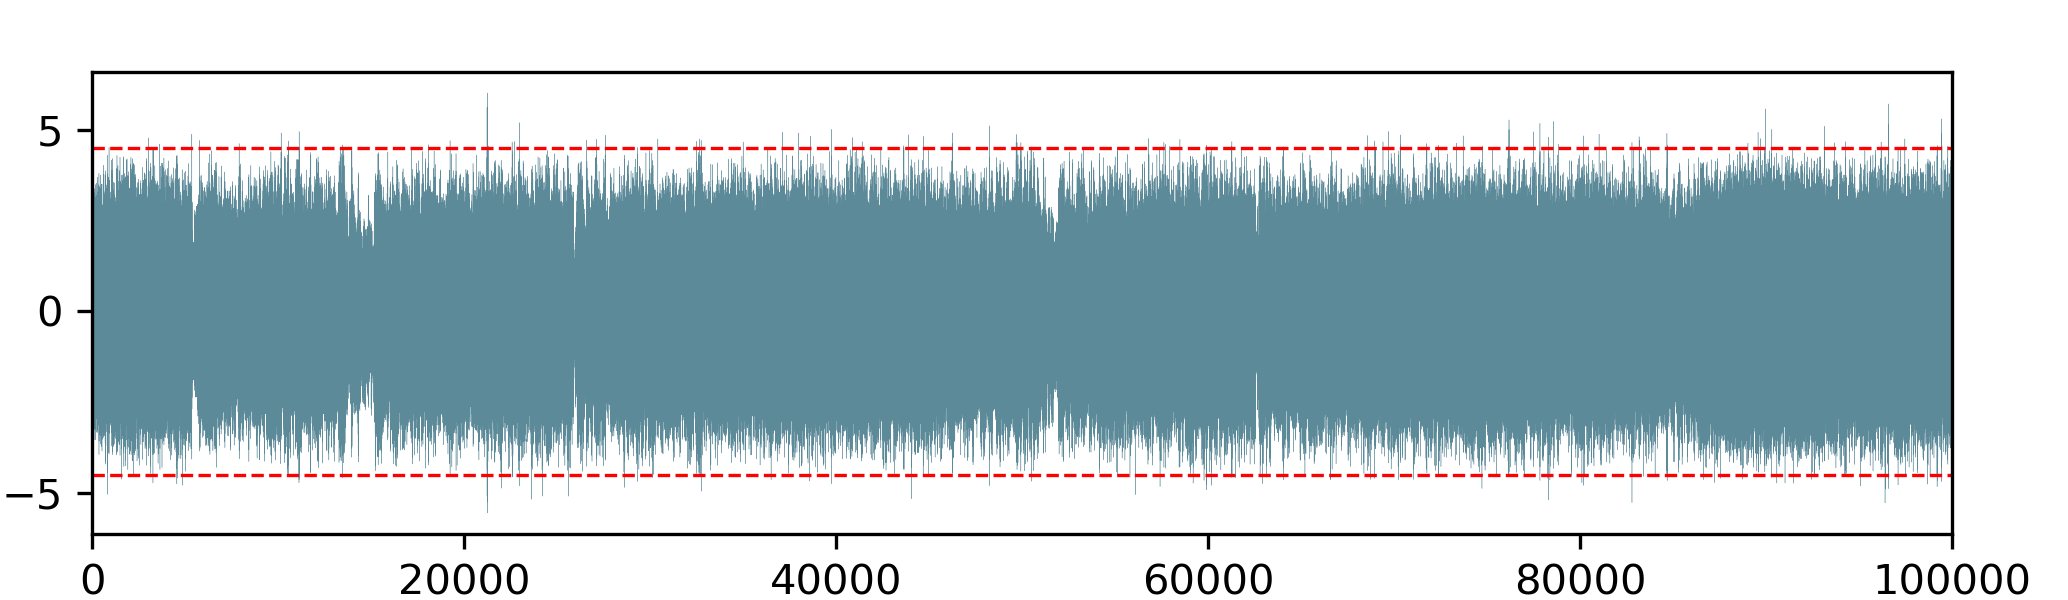
\includegraphics[scale=0.45]{figures/decrypt_tstat.png}
    \label{fig:EMtstat}
\end{figure}

However, similar results are achieved as well on the non-masked version of the algorithms: since other works have proven the existence of 
a power side-channel attack on the RMRS decoder, we conclude that 
further measurements are required to assess the security of the masking scheme.

\subsection{Comparison with other schemes}
    Similarly to the NIST Round 3 report, we can compare the performance of our implementation with the other Round 4 candidates; 
    it is interesting to note that all three candidates are code-based cryptosystems and that they all have a Cortex-M4 implementation.
    In the graphs below we can see the different amount of time required by our implementations, BIKE
    and McEliece to perform the different operations; for consistency, we consider only 
    the optimized implementations for Cortex M4 with level 1 parameters. For HQC, we consider the results
    obtained with zero memory wait states, as the authors of the other implementations did.
        
    \begin{figure*}
        \centering
    \pgfplotstableread[col sep=comma]{ % data 
        Label,     Keygen, Encaps, Decaps
        McEliece, 2146932, 582, 2706
        BIKE, 24935, 3253, 49911
        HQC, 4934, 10441, 15546
        HQC (masked), 8228, 17050, 25522
            }\mydata
        \begin{tikzpicture}
        \centering
        \begin{axis}[
            height=80mm, width=170mm,
    %
            bar width=0.22,
            ybar=0pt,
            enlarge x limits={abs=0.5},
            ymin=0,
            ymax=55000,
            ytick distance=10000,
            yticklabel style={font=\small},
            yticklabel=\pgfmathprintnumber{\tick},
            ylabel={Execution time (kcycles)},
            %xlabel={Cryptosystem},
            xtick=data,
            xticklabels from table={\mydata}{Label},
            grid style={line width=.2pt, draw=gray!20},            
            ymajorgrids=true,
    %
            nodes near coords,
            nodes near coords style={font=\tiny,
                                    /pgf/number format/.cd,
                                                precision=0,
                                                zerofill,
                                    },
        ]
    \addplot[preaction={fill=blue!30}, pattern=north west lines, pattern color=blue!50!black] table [x expr=\coordindex,y=Keygen]{\mydata};
    \addplot[preaction={fill=red!30}, pattern=crosshatch dots, pattern color=purple!70] table [x expr=\coordindex,y=Encaps]{\mydata};
    \addplot[preaction={fill=yellow!30}, pattern=north east lines, pattern color=orange!70] table [x expr=\coordindex,y=Decaps]{\mydata};
    \end{axis}
    \end{tikzpicture}
    
    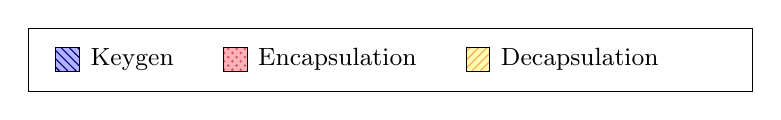
\begin{tikzpicture}
        % draw a rectangle around all
        \draw[fill=white, draw=black] (-0.5, -0.4) rectangle (8.7, 0.4);
        \node [draw, preaction={fill=blue!30}, pattern=north west lines, pattern color=blue!50!black, rectangle, minimum width=0.3cm, minimum height=0.3cm] (box1) {};
        \node [right=0.01cm of box1] (text1) {\small Keygen};
        \node [draw, preaction={fill=red!30}, pattern=crosshatch dots, pattern color=purple!70, rectangle, minimum width=0.3cm, minimum height=0.3cm, right=0.5cm of text1] (box2) {};
        \node [right=0.01cm of box2] (text2) {\small Encapsulation};
        \node [draw, preaction={fill=yellow!30}, pattern=north east lines, pattern color=orange!70, rectangle, minimum width=0.3cm, minimum height=0.3cm, right=0.5cm of text2] (box3) {};
        \node [right=0.01cm of box3] (text3) {\small Decapsulation};
    \end{tikzpicture}
    \caption{Comparison of execution time for the McEliece, BIKE, and HQC KEMs}
    \label{fig:time}
    \end{figure*}

    We can see how the McEliece cryptosystem is the fastest one in terms of encapsulation and decapsulation, but 
    requires $2\cdot 10^{12}$ cycles to generate the keypair. With respect to BIKE, the most promising
    candidate in this round, we can see how HQC outperforms it in terms of key generation and decapsulation,
    not only in the fast implementation but also in the masked one.


    In terms of size, we can see how McEliece is prohibitively large in terms of keysize (over 250KB for the public key only).
    With respect to BIKE, we can see that HQC ciphertext and public keys are larger by a factor of $2.9$ and $1.5$ respectively.

    \begin{figure*}
        \centering
    \pgfplotstableread[col sep=comma]{ % data 
    Label,     pk, sk, ctx
    McEliece, 261120, 6492, 128
    BIKE, 1540, 280, 1572
    HQC, 2249, 40, 4481
        }\memorytable
        \begin{tikzpicture}
        \centering
        \begin{axis}[
            height=80mm, width=150mm,
    %
            bar width=0.22,
            ybar=0pt,
            enlarge x limits={abs=0.5},
            ymin=0,
            ymax=8000,
            ytick distance=1000,
            yticklabel style={font=\small},
            yticklabel=\pgfmathprintnumber{\tick},
            ylabel={Memory usage (Bytes)},
            %xlabel={Cryptosystem},
            xtick=data,
            xticklabels from table={\memorytable}{Label},
            grid style={line width=.2pt, draw=gray!20},            
            ymajorgrids=true,
    %
            nodes near coords,
            nodes near coords style={font=\tiny,
                                    /pgf/number format/.cd,
                                                precision=0,
                                                zerofill,
                                    },
            legend style={legend pos=north east,
                        cells={anchor=west},
                        font=\footnotesize,
                        }
        ]
    \addplot[preaction={fill=blue!30}, pattern=north west lines, pattern color=blue!50!black] table [x expr=\coordindex,y=pk]{\memorytable};
    \addplot[preaction={fill=red!30}, pattern=crosshatch dots, pattern color=purple!70] table [x expr=\coordindex,y=sk]{\memorytable};
    \addplot[preaction={fill=yellow!30}, pattern=north east lines, pattern color=orange!70] table [x expr=\coordindex,y=ctx]{\memorytable};
    \end{axis}
        \end{tikzpicture}
    
        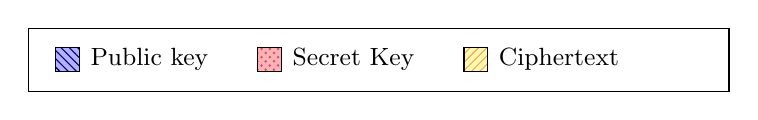
\begin{tikzpicture}
            % draw a rectangle around all
            \draw[fill=white, draw=black] (-0.5, -0.4) rectangle (8.4, 0.4);
            \node [draw, preaction={fill=blue!30}, pattern=north west lines, pattern color=blue!50!black, rectangle, minimum width=0.3cm, minimum height=0.3cm] (box1) {};
            \node [right=0.01cm of box1] (text1) {\small Public key};
            \node [draw, preaction={fill=red!30}, pattern=crosshatch dots, pattern color=purple!70, rectangle, minimum width=0.3cm, minimum height=0.3cm, right=0.5cm of text1] (box2) {};
            \node [right=0.01cm of box2] (text2) {\small Secret Key};
            \node [draw, preaction={fill=yellow!30}, pattern=north east lines, pattern color=orange!70, rectangle, minimum width=0.3cm, minimum height=0.3cm, right=0.5cm of text2] (box3) {};
            \node [right=0.01cm of box3] (text3) {\small Ciphertext};
        \end{tikzpicture}
        \caption{Memory usage comparison of McEliece, BIKE and HQC}
        \label{fig:memory}
    \end{figure*}

\section{Conclusions}
In this thesis we provided the first constant-time implementation of HQC and the
first masked implementation of HQC's public key encryption scheme.

To do so, we evaluated different multiplication methods in terms of both performance and constant-time behavior, 
crowning the Frobenius Additive FFT as the best one on the ARM Cortex-M4 and the Karatsuba algorithm on x86 architectures;
moreover, we implemented a masking scheme for the key generation, encryption and decryption primitives
of HQC's public key encryption scheme.

We provided a comparative analysis of the Round 4 NIST PQC candidates, showing how both our constant-time and masked implementations 
of HQC offer a good trade-off in terms of memory consumption and execution time, being faster than the (unmasked) BIKE implementation
and thus making them suitable for standardization.

As future work, it could be possible to run more accurate tests in order to evaluate the efficacy of our masking scheme against power attacks.
Since our masking scheme targets the PKE only, it could also be possible to extend the masking scheme to 
the SHAKE functions and make the whole KEM secure against power attacks.

%---------------------------------------------------------------------------
%  BIBLIOGRAPHY
%---------------------------------------------------------------------------
% Remember to insert here only the essential bibliography of your work
\bibliography{refs.bib} % automatically inserted and ordered with this command 

\end{document}